%% sample template file for a MSc Thesis
%% The default is with two sided setup:
\documentclass[%
oneside,    %% uncomment for onesided layout
project,    %% uncomment not thesis but project report
nosummary   %% uncomment if no summary page should be generated
]{USN-MSc}

% The following command removes the chapter names form the header
% (comment/remove) if you prefer to have them:
\pagestyle{plain}

% --- Bibliography setup ---
%%% default is the "ieee" style
\usepackage[style=ieee, sorting=none]{biblatex}
%%% If you want to use "author-year" style
%%% where `\cite{Foo2011}` generates "Foo et al. (2011)"
%%% and   `\parencite{Foo2011}` generates "(Foo et al. 2011)"
%%% then comment the line above and use
%\usepackage[style=authoryear]{biblatex}
%%% or
%%% if you want to use "alphabetic" style then use
%%% where `cite[Foo2011]` generates "[Foo11]"
%%% then comment the line above and use
%\usepackage[style=alphabetic]{biblatex}
%%% instead.
%% load the bib file:
\addbibresource{MScThesis.bib}

\usepackage{lipsum} % just for providing fill text used in this template
\usepackage{array} % for adjusting tables?
\usepackage{pdflscape} % for landscape pages

%These two are used to add frames to figures.
\usepackage{graphicx}
\usepackage[export]{adjustbox}

% --- general setup ---
%% Please fill in the following parameters:
\newcommand{\mytitle}{%
%% title:
Assignments for section 3 (W3.1-W3.5)
}

\newcommand{\mysubtitle}{%
%% master programme (for thesis only)
%% uncomment the appropriate one:
%%Electrical Power Engineering
%Energy and Environmental Technology
%Industrial IT and Automation
%Process Technology
}

\newcommand{\mykeywords}{%
%% keywords (for thesis only):
<keyword one, keyword two, \ldots>
}

\newcommand{\myauthor}{%
%% author(thesis) or group code (project):
223786 Lars Rikard Rådstoga
}

\newcommand{\myparticipants}{
%% group participants (for project only)
<First participant>\\
<Second participant>\\
<Third participant>\\
<Fourth participant>
}

\newcommand{\supervisor}{%
%% supervisor:
<Supervisor's Name>}

\begin{document}

% --- title page setup ---
%\USNtitlepage%
%%% Please provide the following information:
%%% #1 optional figure (set to {} if not wanted)
%{%
%  {\normalsize}
%  \begin{figure}[!ht]
%    \centering
%   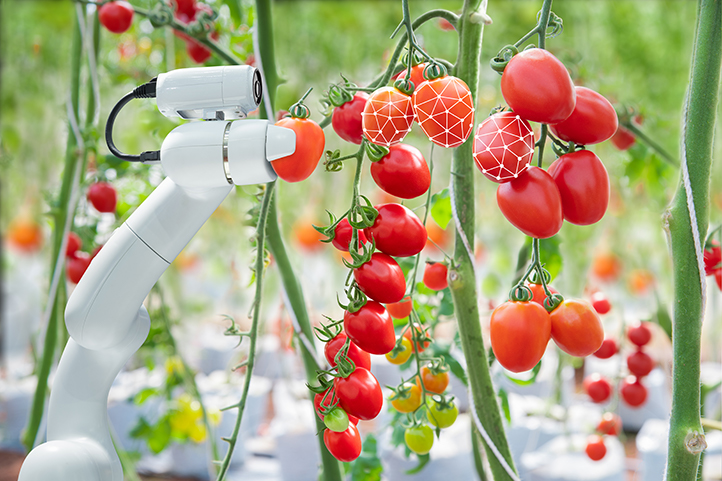
\includegraphics[width=0.8\textwidth]{TomatoPickerBot}
%   \label{fig:tomatoBot}
% \end{figure}
%}
% --- title page setup ---
\USNtitlepage%
%% Please provide the following information:
%% #1 optional figure (set to {} if not wanted)
{%
  {\normalsize}
   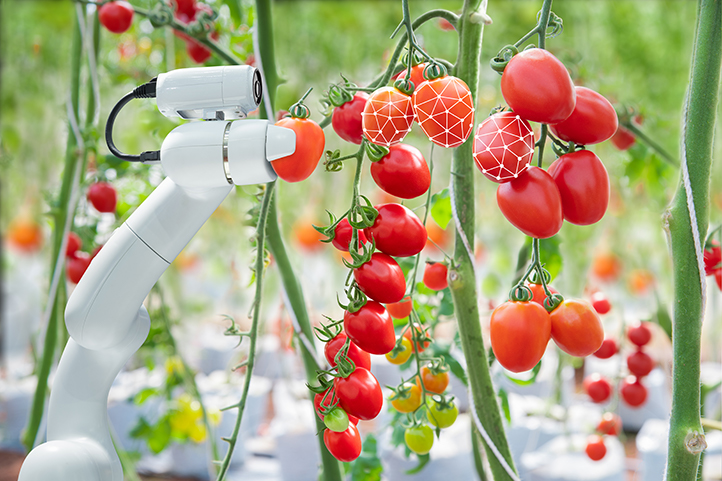
\includegraphics[width=\textwidth]{TomatoPickerBot}}
%% #2 Project partner:
{<Project partner>}
%% #3 Summary:
{%
\lipsum[6-7]
}


%\chapter*{Preface}
%\label{ch:preface}
%\addcontentsline{toc}{chapter}{Preface}
%\lipsum[1-3]
%\bigskip
%Porsgrunn, \today

%\myauthor %% for thesis
%\myparticipants %% for project


%% table of contents
\tableofcontents
\addcontentsline{toc}{chapter}{\contentsname}

%\listoffigures % out-comment if unwanted
%\addcontentsline{toc}{section}{\listfigurename}

%\listoftables  % out-comment if unwanted
%\addcontentsline{toc}{section}{\listtablename}

\chapter{System diagram for the chosen autonomous system}
\label{ch:sysDiagram}
This chapter contains context of the autonomous fruit picker system. Briefly discussing why it should be an autonomous system and how it should be organized in terms of building blocks and how data should flow through the system.
\section{Introduction of the system}
The autonomous fruit picker system is meant to be a contribution to combat increasing shortage in labor in the agricultural landscape. As fruit picking is tedious and back-breaking work it is not the most lucrative profession. Most robotized fruit-picking solutions as of today involve augmentation of the farming environment to a great degree, such as moving the operation in-doors or levitating the farming beds. Perhaps these augmentations are advantageous for tackling multiple challenges, but they might have their downsides as well. Today we are going to assume that traditional outdoor ground farming is the most popular practice and will remain that way for most of the foreseeable future. The target environment for the system will therefore be a more rugged and unpredictable one compared to environments in which existing solutions operate.
\section{System diagram}
Based on system architecture theory from the book Introduction to AI Robotics \cite{murphy2000introduction}, the system will be organized by the five subsystems as seen in figure \ref{fig:sysDiagram}.
\begin{figure}[!ht]
  \centering
  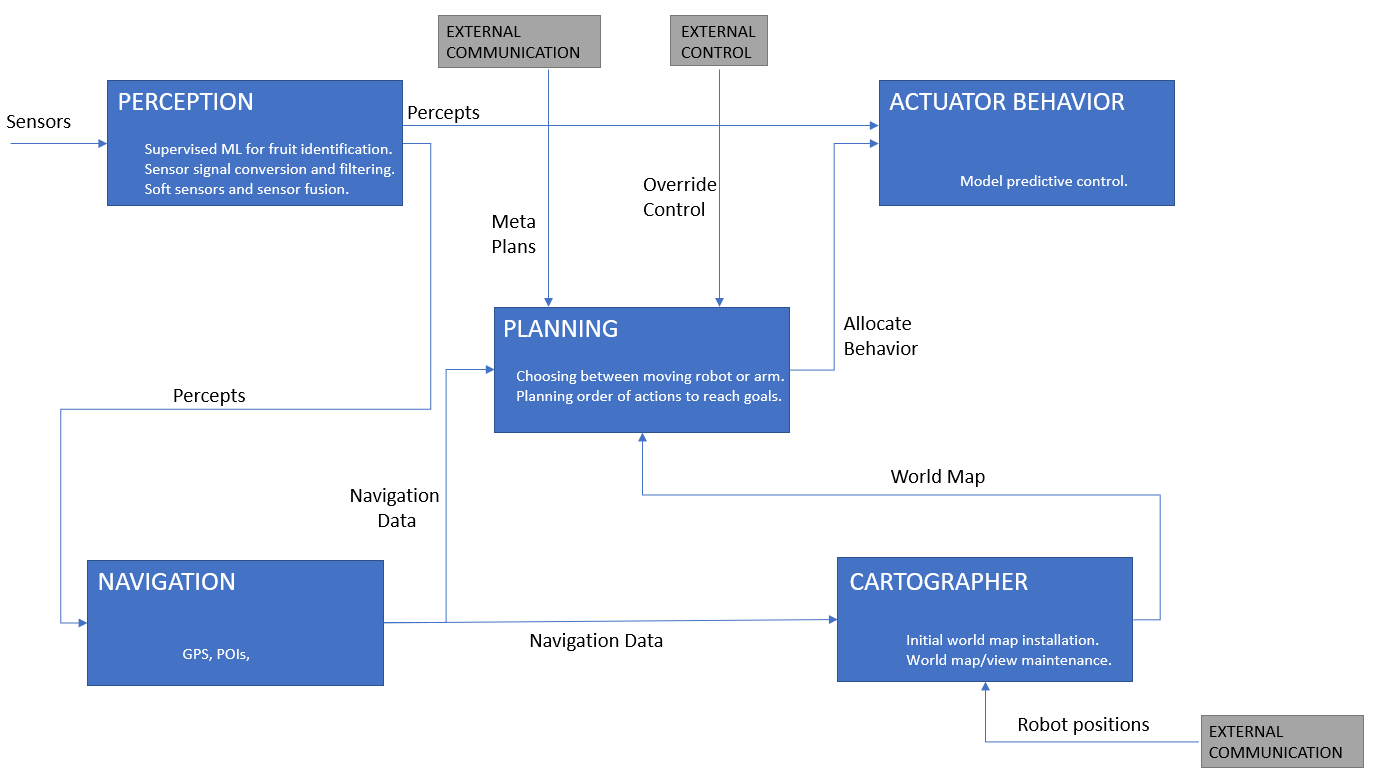
\includegraphics[width=0.95\textwidth, frame]{SystemDiagram}
  \caption{System diagram with focus on data input and internal data flow. \cite{murphy2000introduction}}
  \label{fig:sysDiagram}
\end{figure}
In order for a system to traverse a world, several cognitive modules need to cooperate. As described in the literature, there are usually a minimum of five of these modules or subsystems: perception, navigation, planning, cartographer, and motor schema. In the aforementioned system diagram, shown in this paper, motor schema is instead named actuator behavior. These subsystems will be made up of one or more classes in object-oriented programming. For this solution it is plausible that different implementations of these subsystems will be required for the robot's main body and the gripper-equipped arm.

The perception subsystem is tightly-knit together with the sensor inputs. Sensors will supply the system with a continuous stream of information about the surrounding world: tactile feedback, LIDAR, camera, GPS, wheel rotation encoder, and more. Analog data will have to be converted to digital and raw data will need to be filtered. Redundant sensors can be combined to increase accuracy or different kinds of sensors can be combined: fused. ML models trained for identification can also be part of this subsystem. Most important is the model for identifying and differentiating fruit.

The navigation subsystem will be responsible for planning and monitoring movement of the robot. This module will however require data from related modules: transformed sensor data from the perception module, map data from the cartographer and plans from the planning module. Initially the planning module will decide where the robot should move, the cartographer will have partial data about surrounding world. The navigation module will use this data to calculate and iteratively re-calculate optimal paths. If the cartographer discovers some obstacles in the way of the planned path the navigator might require major re-routing. Additionally, perceptive signals can be used directly for collision detection. If something unexpected moves in the way of the robot, the sensors will pick this disturbance up before it is mapped by the cartographer.

The planning subsystem will be the main local decision maker for the robot. Its main tasks involve planning such as what area to pick fruit from during spans of hours, managing the order of main activities such as moving to a bush, drop-off area, picking fruit, charging, and more. A more macro level of decision-making is made in a centralized server, so this will be important inputs for the module. But it will also need to look at reception data, such as how many fruit are visible, to e.g. micromanage between moving the robot and picking fruit. Such information will also be communicated to the server to further adjust macro management.

The cartographer subsystem will both use perceptive data to map the world, but it will also communicate with other units through the central server to build a more detailed map.

The actuator subsystem will use both navigation data, perceptive data and control algorithms such as PID, LQI, or MPC to control the robot.

\chapter{How to organize software for autonomous systems}
\label{ch:softOrganz}
This chapter contains information on the organization of software in the autonomous system.
\section{Reflection}
The system will be distributed into three different layers, see figure \ref{fig:layers}.
From the ground-up: multiple robots can operate independently and run their own code, a common server will be the responsible for macro planning, communication between robots, collecting data, training ML models and distributing updated software. Additionally, the system requires a database for saving sensory data, world views, and other resources that can be used to further improve the system or that create value in other ways.

\begin{figure}[!ht]
  \centering
  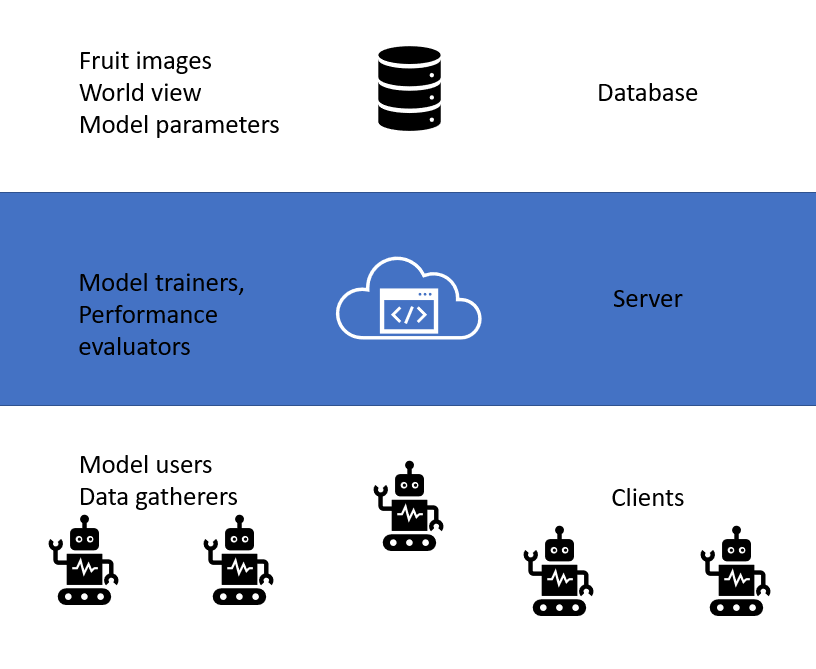
\includegraphics[width=0.80\textwidth, frame]{SystemLayers}
  \caption{Layered architecture displaying multiple robots communicating through a common server and database.}
  \label{fig:layers}
\end{figure}

\chapter{Information collection}
\label{ch:infoCol}
This chapter contains a discussion on collection of information.
\section{Reflection}
Information from sensors will be saved to the database from the server. There might be a need to supplement datasets by labeling more fruit of different states.


\chapter{Learning}
\label{ch:learn}
This chapter contains a reflection on the use of learning in the autonomous system.
\section{Reflection}
Learning should be used to train multiple required models used inside the robot. Camera and arm coordination, fruit identification, traversal, and more.

% A dummy command that causes all bibliographyentries to be displayed
% even though there were not cited in the document. Used for demonstration
% purposes only in this template file.
~\nocite{*}

\cleardoublepage

% The bibliography should be displayed here...
%\printbibliography[heading=bibintoc]
% You rather like to call the bibliography "References"? Then use this instead:
\printbibliography[heading=bibintoc, title={References}]


%\appendix
%\renewcommand{\appendixname}{Paper} %% So we get 'Paper X' displayed instead


%\chapter[Short Title of Paper A]{Title of Paper A (probably very long and therefore not good to have in the header)}
%\label{paper-a}
%
%\paragraph{Note}
%Since some papers tend to have a rather long title it is good to provide the optional short title which then will be displayed in the table of contents and header instead of the long original title.
%On the openening page of the chapter the orginal \emph{long} title will be displayed.\bigskip
%
%\emph{Short descriptive text of paper follows here.}\bigskip
%
%The paper itself needs to be included in the published form as PDF on the next pages.
%This can be done using the \texttt{pdfpages} package by adding the command:
%
%\begin{verbatim}
%\includepdf{pages=-,openright}{Filename}
%\end{verbatim}
%
%You can omit the \texttt{.pdf} when specifying the \texttt{Filename}. Also you should include always include the option \texttt{openright} since it would look strange to have the paper starting at the back of the cover page.
%
%There are more options like only adding specific pages:
%\begin{verbatim}
%\includepdf{pages=2-6,openright}{Filename.pdf}
%\end{verbatim}

%For more options see Appendix~\ref{paper-b} where the most important pages of the \texttt{pdfpages} manual were inlcuded using \texttt{pdfpages}.


%%% Command to include a PDF file directly including all pages:


%\chapter[Short Title of Paper B]{Title of Paper B}
%\label{paper-b}
%Short descriptive text of paper follows here.
%
%Here we included the first five pages of the \texttt{pdfpages} manual itself.
%
%\includepdf[pages=1-5,openright]{fig/pdfpages}
%
\end{document}

%%% Local Variables:
%%% mode: latex
%%% TeX-master: t
%%% End:
